\documentclass[a4paper,14pt]{extarticle}

\usepackage[T2A]{fontenc}
\usepackage[utf8]{inputenc}
\usepackage[russian]{babel}
\usepackage{geometry}
\usepackage{xcolor}
\usepackage{listings}
\usepackage{hyperref}
\usepackage{longtable}
\usepackage{graphicx}
\usepackage{xurl}

\geometry{left=25mm,right=15mm,top=20mm,bottom=20mm}
\hypersetup{colorlinks=true,linkcolor=black,urlcolor=blue}

\lstdefinestyle{javastyle}{
    basicstyle=\ttfamily\small,
    breaklines=true,
    frame=single,
    tabsize=4,
    showstringspaces=false,
    keywordstyle=\color{blue!60!black},
    commentstyle=\color{green!40!black},
    stringstyle=\color{red!50!black},
    numbers=left,
    numberstyle=\tiny,
    inputencoding=utf8,
    extendedchars=true
}

\lstdefinestyle{yamlstyle}{
    basicstyle=\ttfamily\small,
    breaklines=true,
    frame=single,
    tabsize=2,
    showstringspaces=false,
    numbers=left,
    numberstyle=\tiny,
    inputencoding=utf8,
    extendedchars=true
}

\lstset{style=javastyle}

\newcommand{\screenshot}[3]{
    \begin{figure}[h]
        \centering
        \IfFileExists{#1}
            {\includegraphics[width=#2\linewidth]{#1}}
            {\fbox{\parbox{0.86\linewidth}{\centering
                Место для скриншота: \texttt{\detokenize{#1}}\\[2mm]#3}}}
        \caption{#3}
    \end{figure}
}

\begin{document}

\begin{titlepage}
    \centering
    {\large Университет ИТМО\par}
    \vspace{3cm}
    {\Large Дисциплина: <<Веб-программирование>>\par}
    \vspace{1cm}
    {\LARGE Отчёт по лабораторной работе №4\par}
    \vspace{2cm}
    \begin{flushright}
        Студент: Шубин Егор Вячеславович\\
        Группа: P3209\\
        Вариант: 57441
    \end{flushright}
    \vfill
    Санкт-Петербург\\
    2026
\end{titlepage}

\tableofcontents
\newpage

\section{Текст задания}
\begin{figure}[h]
    \centering
    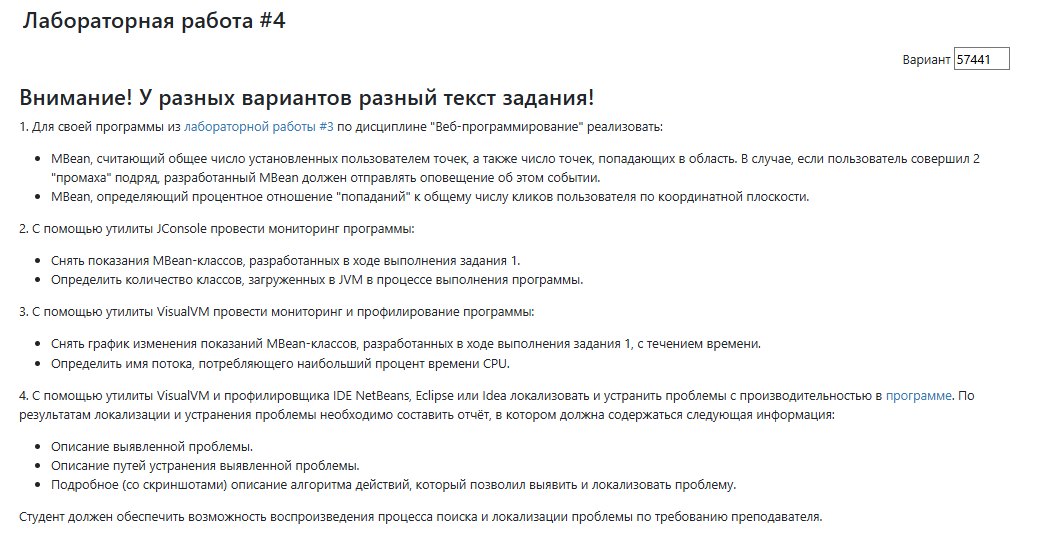
\includegraphics[width=1\linewidth]{task.png}
    \caption{Задание}
    \label{fig:placeholder}
\end{figure}

\section{Листинг программы}
{\href{https://github.com/sshubuntu/OPI_lab4}{\underline{Код программы}}}
\newpage
\section{Jconsole}
\subsection{Метаданные Mben'ов}
\begin{figure}[h]
    \centering
    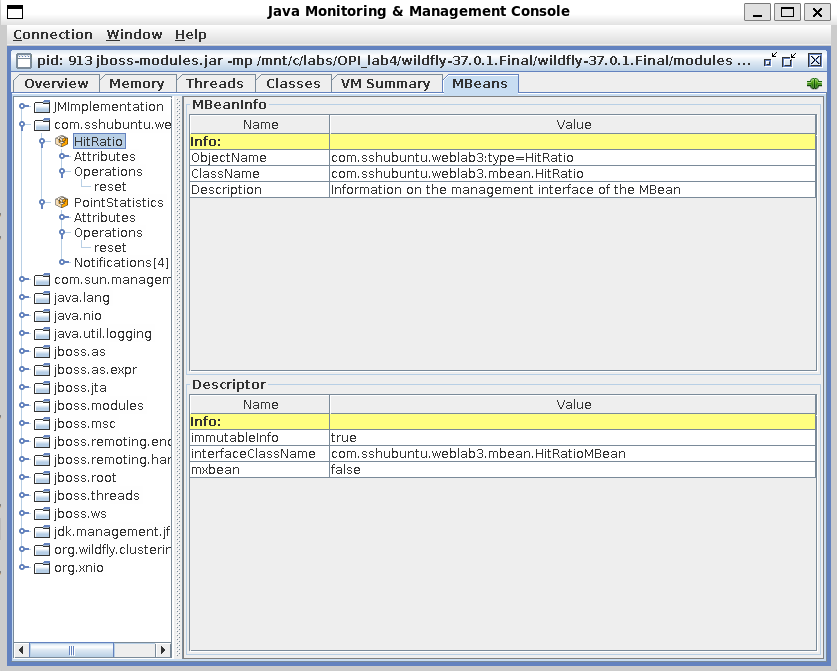
\includegraphics[width=0.62\linewidth]{meta1.png}
    \caption{HitRatio}
    \label{fig:placeholder}
\end{figure}

\begin{figure}[h]
    \centering
    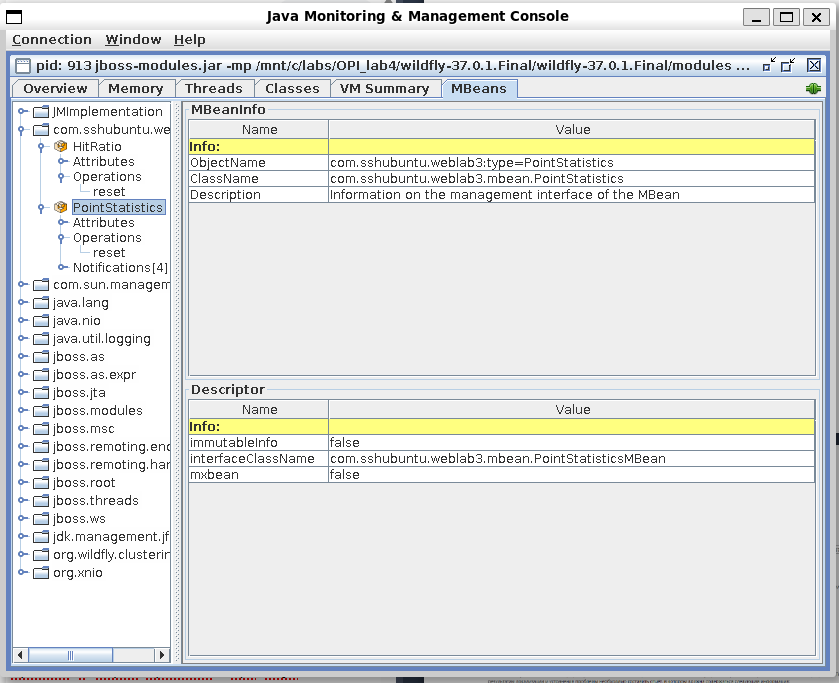
\includegraphics[width=0.62\linewidth]{meta2.png}
    \caption{PointStatistics}
    \label{fig:placeholder}
\end{figure}
\newpage
\subsection{Показания Mben'ов}
\begin{figure}[h]
    \centering
    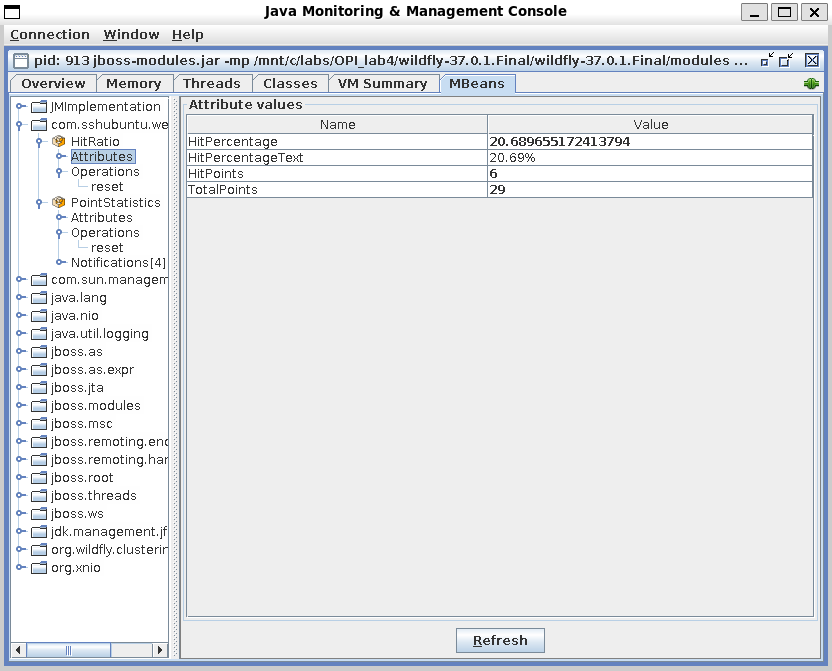
\includegraphics[width=0.6\linewidth]{attributes1.png}
    \caption{HitRatio}
    \label{fig:placeholder}
\end{figure}

\begin{figure}[h]
    \centering
    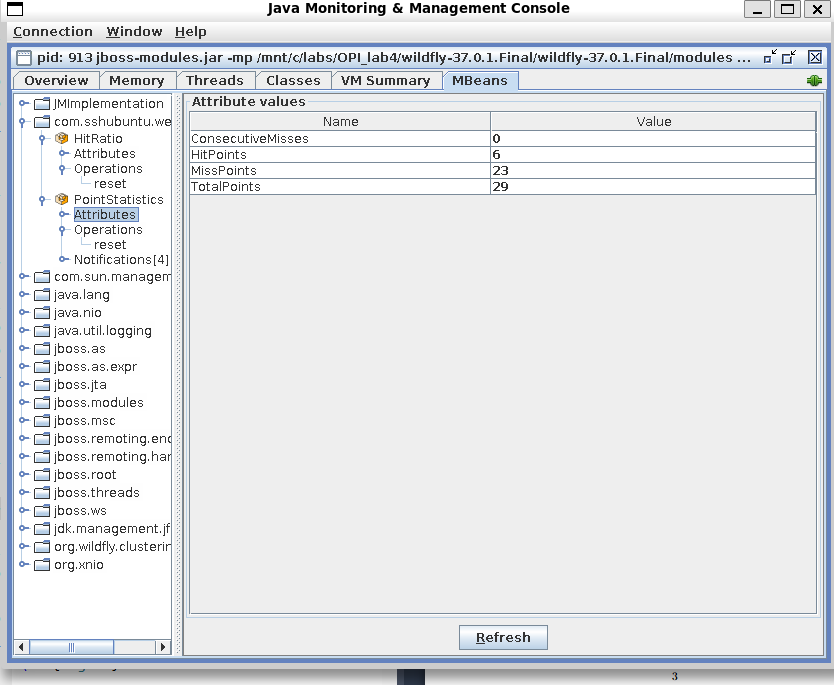
\includegraphics[width=0.6\linewidth]{attributes2.png}
    \caption{PointStatistics}
    \label{fig:placeholder}
\end{figure}
\newpage
\subsection{Графики}
\begin{figure}[h]
    \centering
    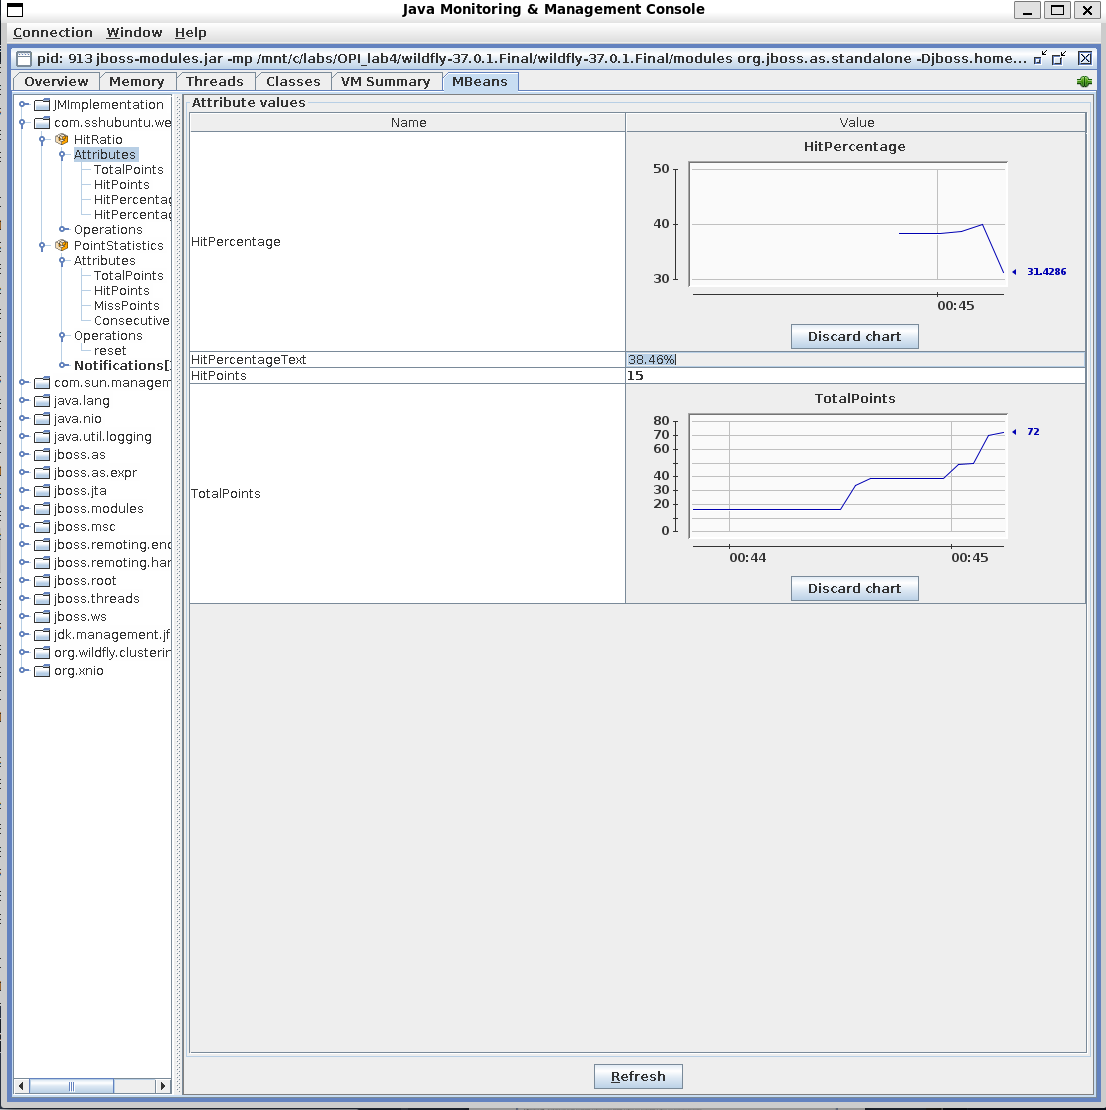
\includegraphics[width=0.5\linewidth]{graph1.png}
    \caption{HitRatio}
    \label{fig:placeholder}
\end{figure}

\begin{figure}[h]
    \centering
    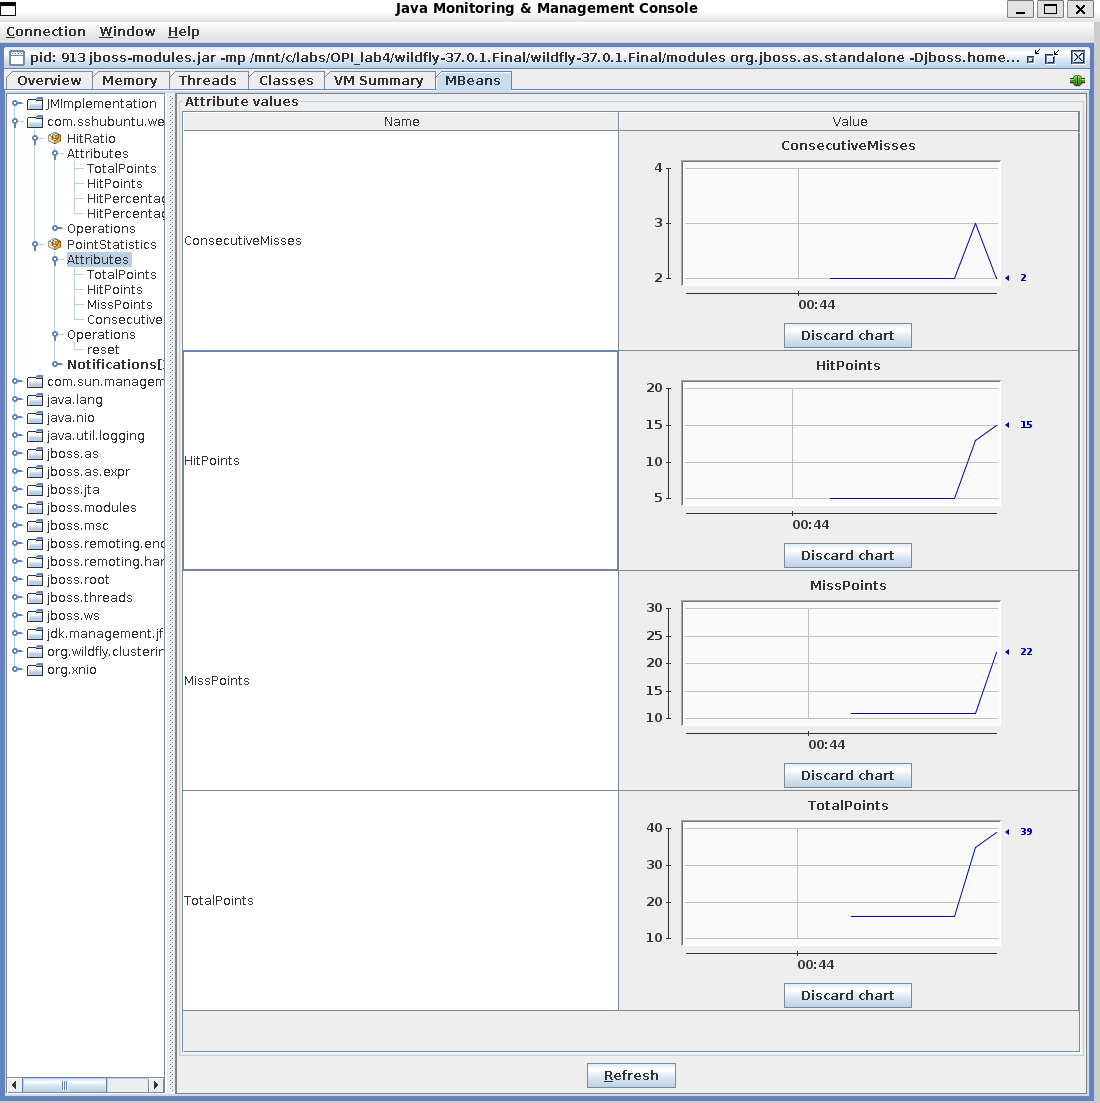
\includegraphics[width=0.5\linewidth]{graph2.png}
    \caption{PointStatistics}
    \label{fig:placeholder}
\end{figure}

\newpage
\subsection{Уведомления}
\begin{figure}[h]
    \centering
    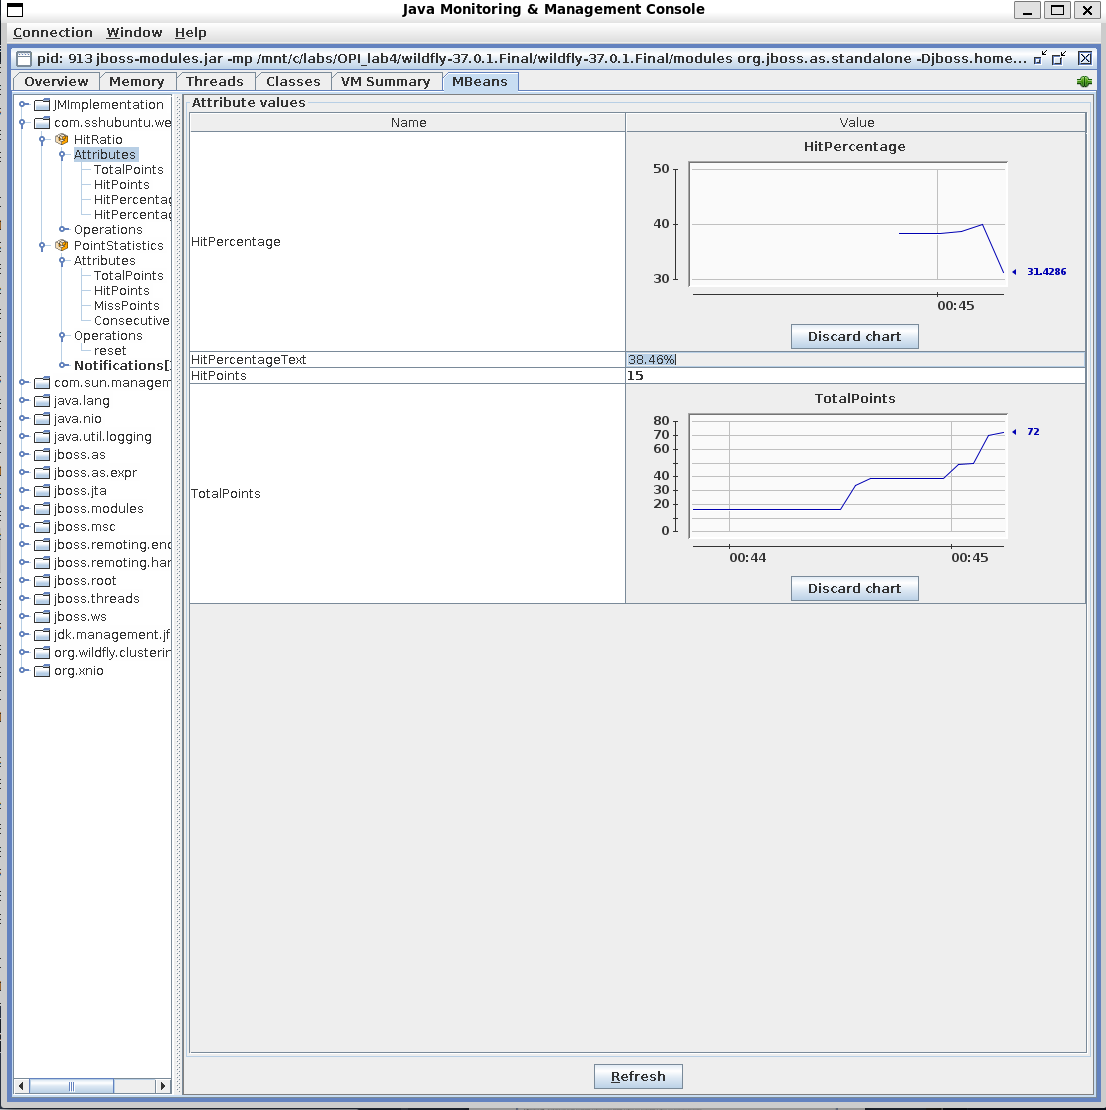
\includegraphics[width=0.4\linewidth]{graph1.png}
    \caption{PointStatistics}
    \label{fig:placeholder}
\end{figure}
\subsection{Кол-во классов}
\begin{figure}[h]
    \centering
    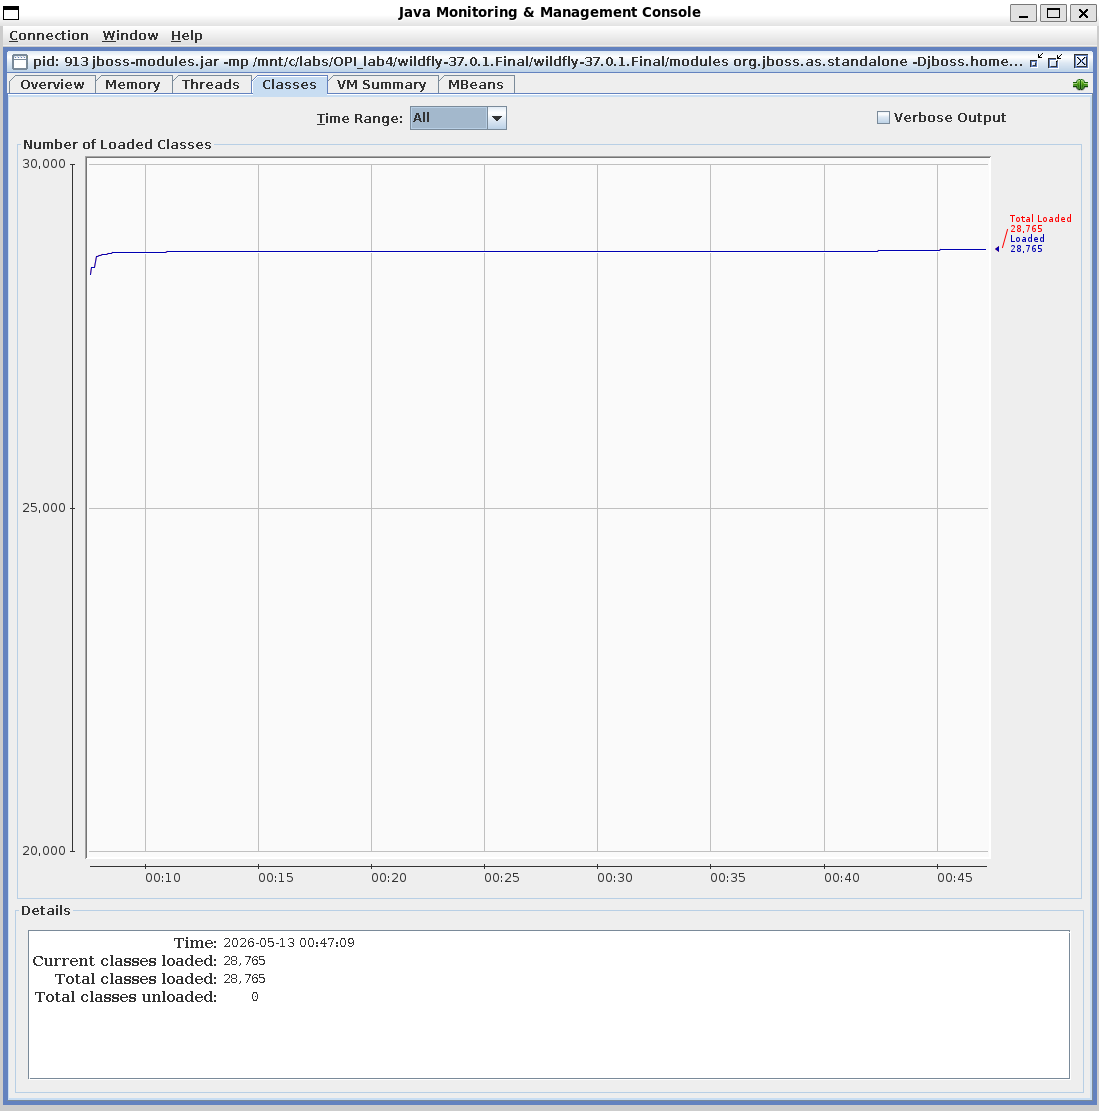
\includegraphics[width=0.5\linewidth]{ClassCount.png}
    \caption{Количество загруженных классов}
    \label{fig:placeholder}
\end{figure}

\subsection{Вывод по разделу}

В JConsole были успешно обнаружены оба разработанных MBean. Снятые значения атрибутов подтвердили, что счётчики общего числа точек, попаданий, промахов и процент попаданий изменяются после пользовательских кликов.

Графики показали динамику изменения MBean-показателей во времени, а подписка на уведомления подтвердила отправку события при двух промахах подряд. Также через стандартный MBean \texttt{ClassLoading} было определено количество классов, загруженных в JVM.

\newpage
\section{VisualVM}
\subsection{Графики}
\begin{figure}[h]
    \centering
    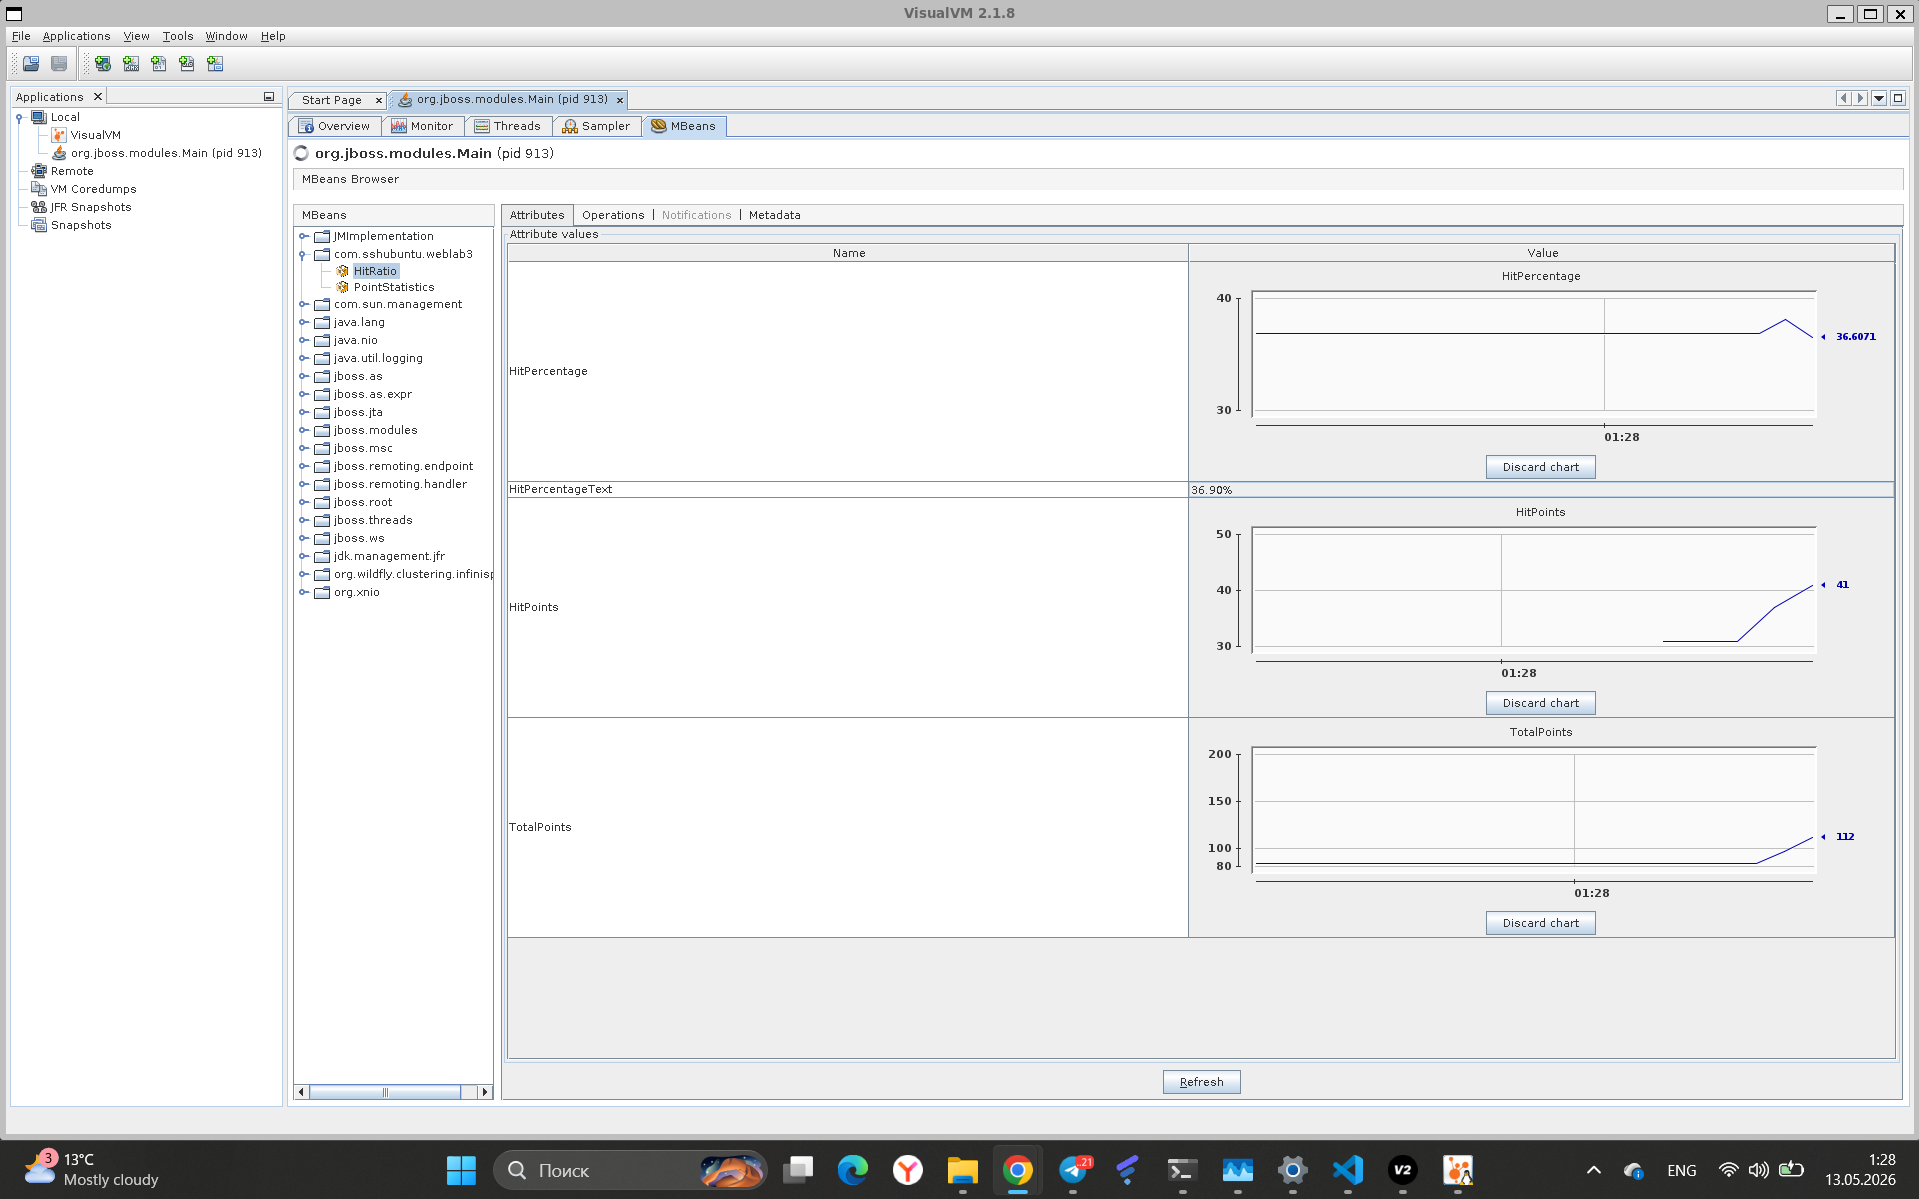
\includegraphics[width=0.7\linewidth]{vis_graph1.png}
    \caption{HitRatio}
    \label{fig:placeholder}
\end{figure}
\begin{figure}[h]
    \centering
    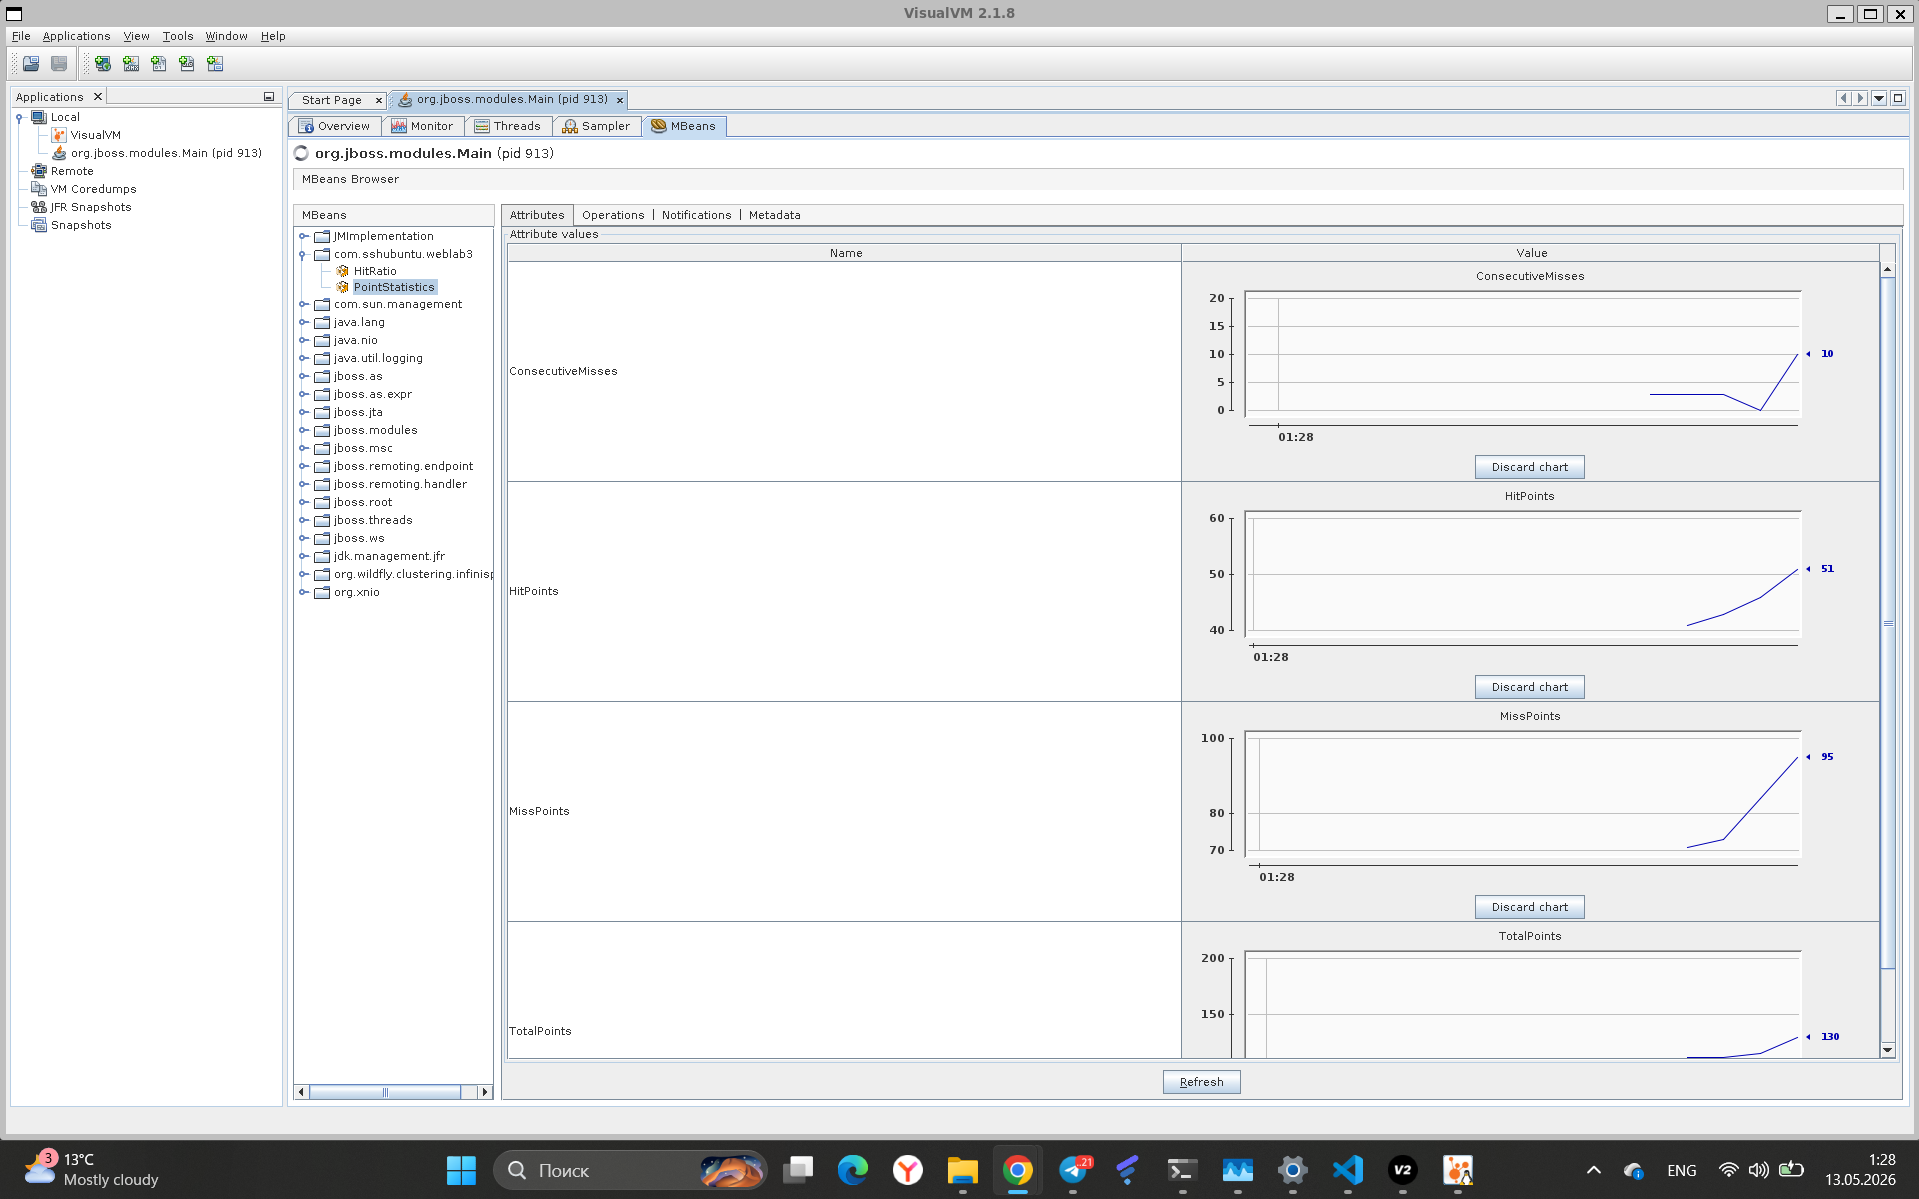
\includegraphics[width=0.7\linewidth]{vis_graph2.png}
    \caption{PointStatistics}
    \label{fig:placeholder}
\end{figure}
\newpage
\subsection{Топ потоков}
\begin{figure}[h]
    \centering
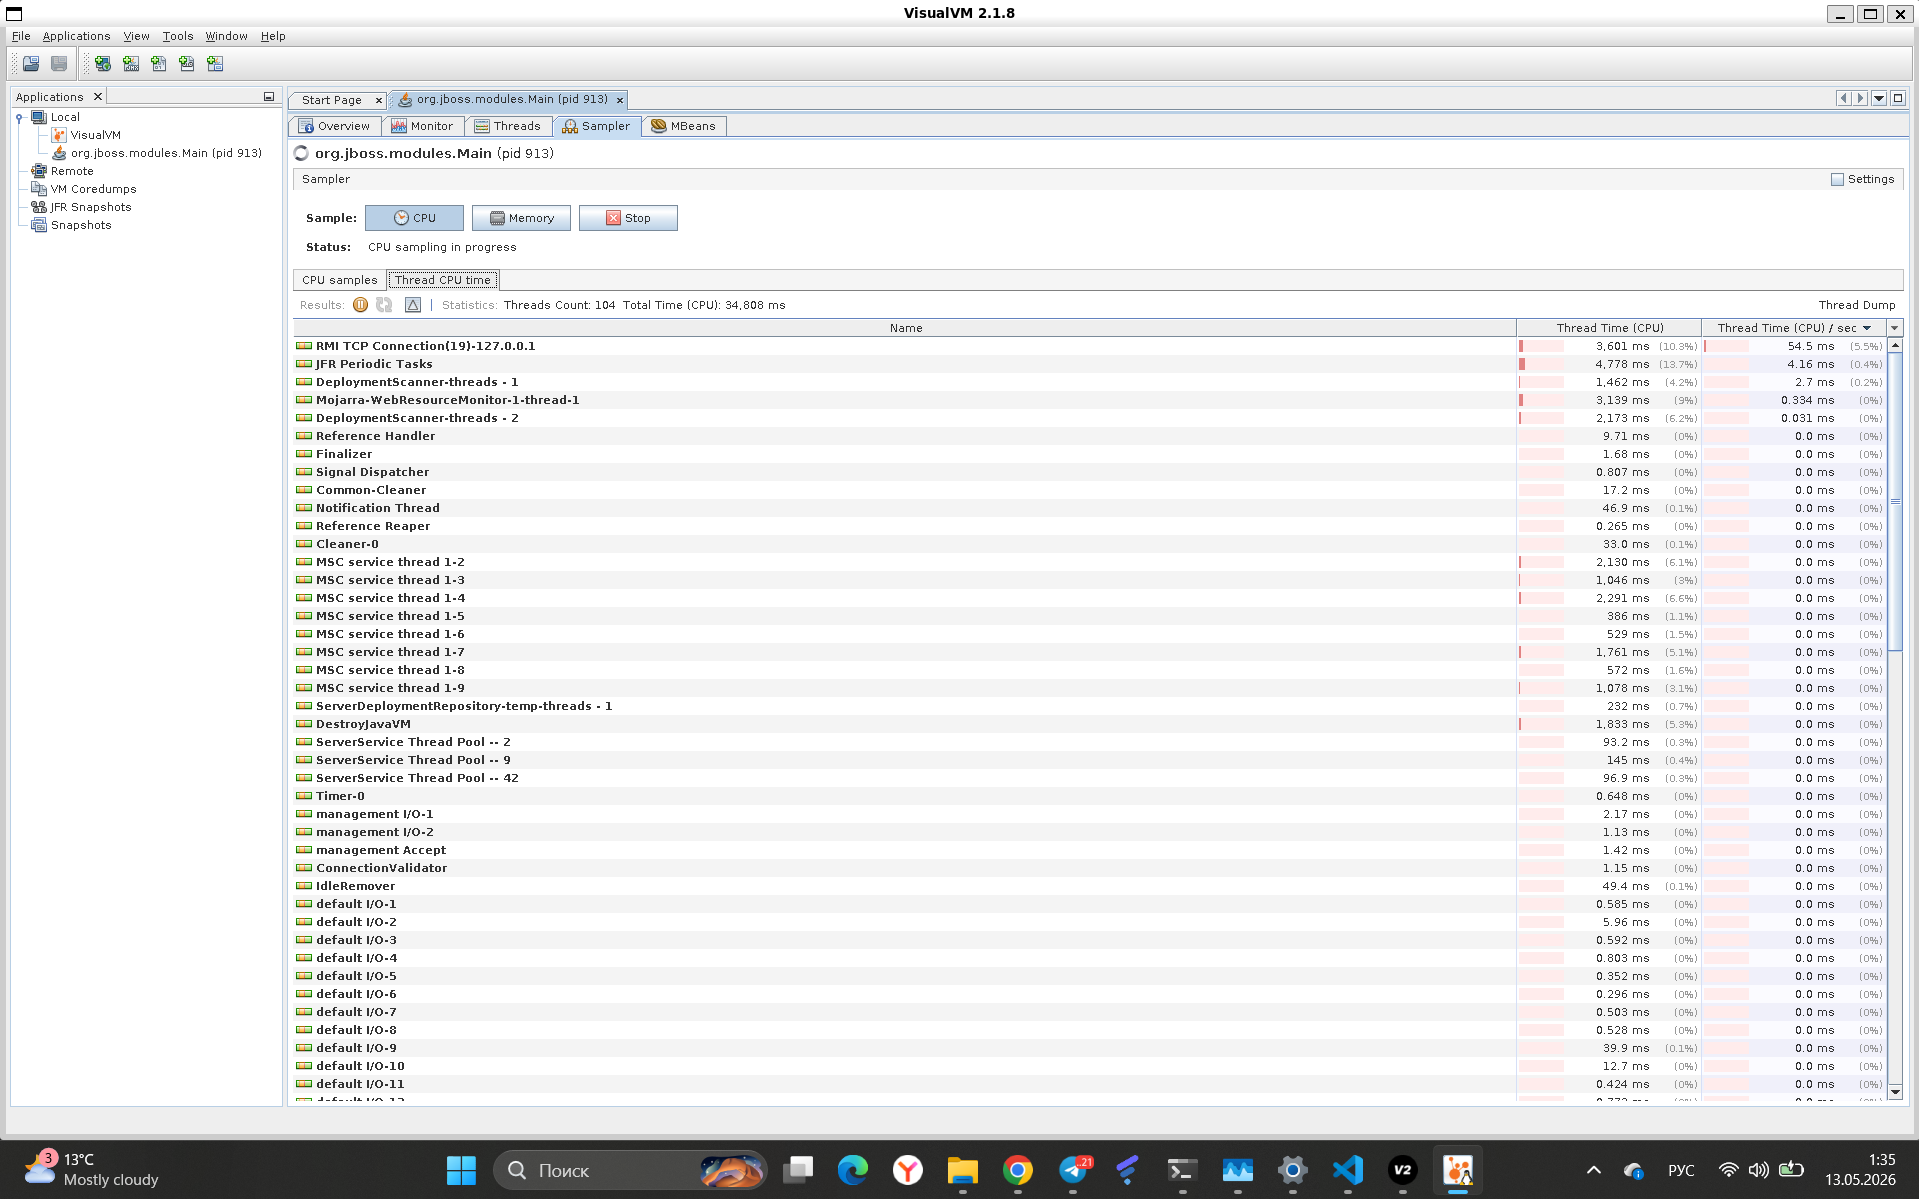
\includegraphics[width=1\linewidth]{threads.png}
    \caption{}
    \label{fig:placeholder}
\end{figure}

\subsection{Вывод по разделу}

В VisualVM были сняты графики изменения показаний MBean во времени. По ним видно, что значения MBean обновляются во время работы приложения и отражают действия пользователя на координатной плоскости.

CPU-профилирование позволило определить поток, потребляющий наибольшую долю процессорного времени. Таким образом, VisualVM был использован не только для мониторинга пользовательских MBean, но и для анализа нагрузки JVM по потокам.

\newpage
\section{Профилирование HttpUnit}
\subsection{Описание выявленной проблемы}

В ходе профилирования была выявлена ошибка производительности, которая заключалась в  утечке в области Metaspace.
На графике Classes наблюдался рост количества загруженных классов, а на графике Metaspace —  увеличение обьема выделенной памяти.
\begin{figure}[h]
    \centering
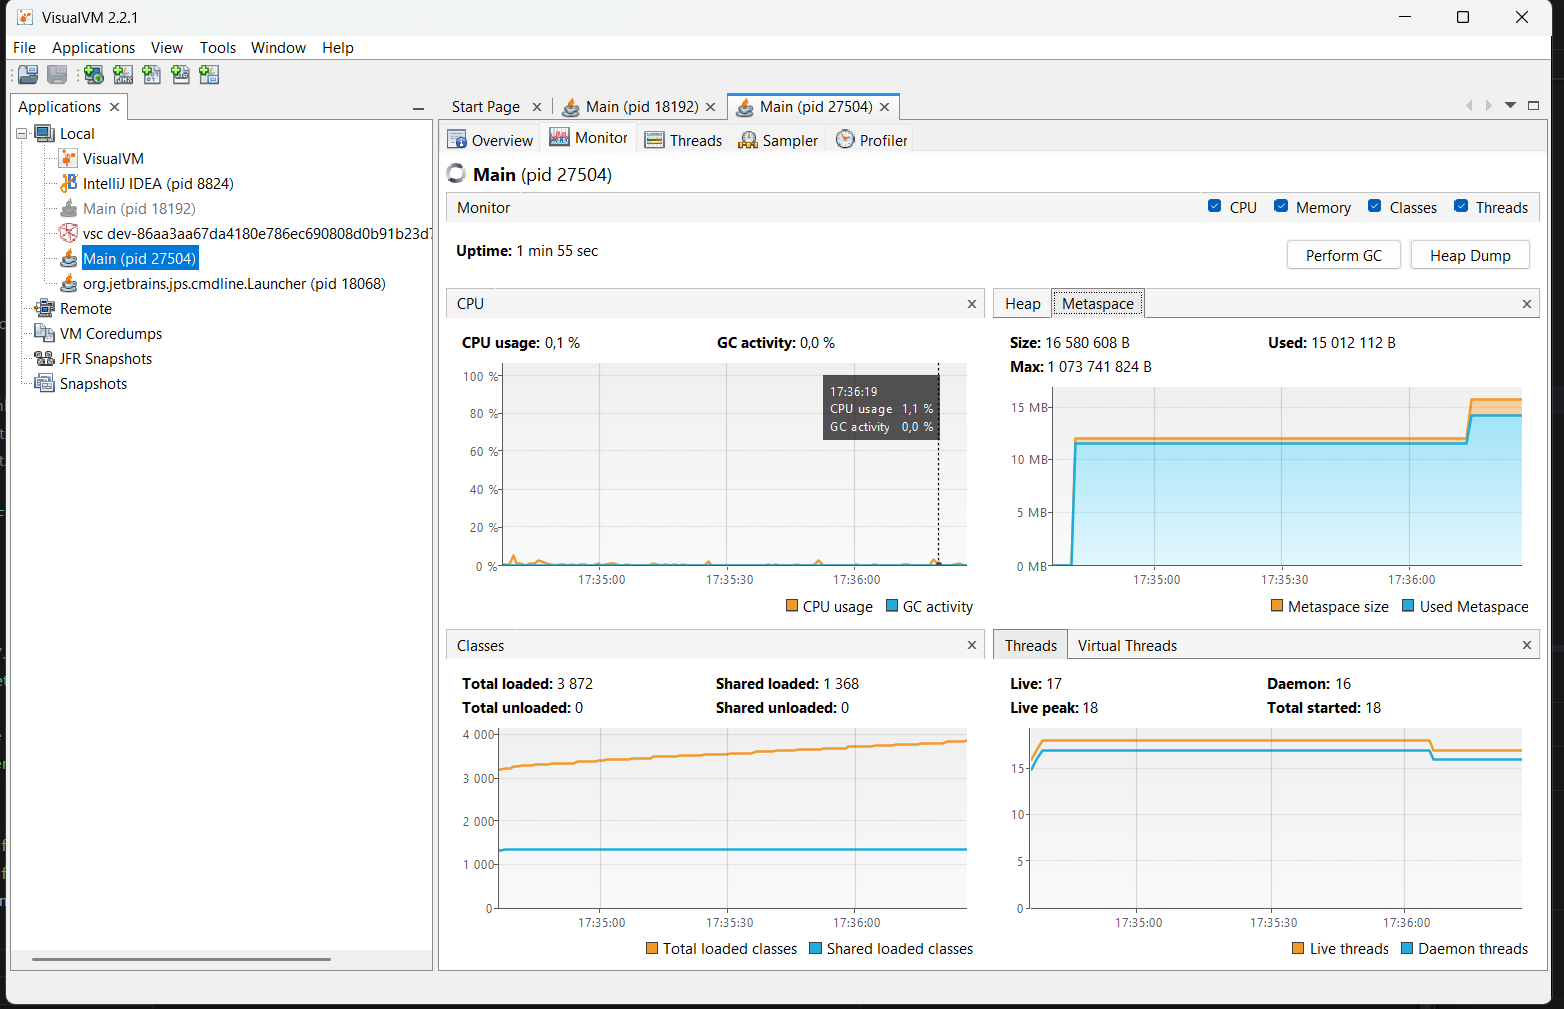
\includegraphics[width=1\linewidth]{metaspace.png}
    \caption{}
    \label{fig:placeholder}
\end{figure}


\end{document}
